%-*-latex-*-
\begin{center}
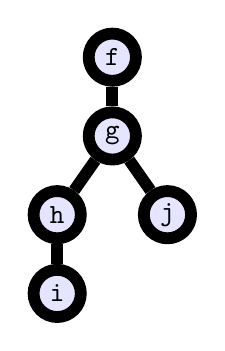
\begin{tikzpicture}

\fill[blue!10] (0.7, 0.0) circle (0.3);
\node [line width=0.15cm,black,minimum size=0.6cm,draw,circle] at (0.7,0.0)(A){};\draw (0.7, 0.0) node[color=black] {\texttt{f}};
\fill[blue!10] (0.7, -1.0) circle (0.3);
\node [line width=0.15cm,black,minimum size=0.6cm,draw,circle] at (0.7,-1.0)(B){};\draw (0.7, -1.0) node[color=black] {\texttt{g}};
\fill[blue!10] (0.0, -2.0) circle (0.3);
\node [line width=0.15cm,black,minimum size=0.6cm,draw,circle] at (0.0,-2.0)(C){};\draw (0.0, -2.0) node[color=black] {\texttt{h}};
\fill[blue!10] (0.0, -3.0) circle (0.3);
\node [line width=0.15cm,black,minimum size=0.6cm,draw,circle] at (0.0,-3.0)(D){};\draw (0.0, -3.0) node[color=black] {\texttt{i}};
\fill[blue!10] (1.4, -2.0) circle (0.3);
\node [line width=0.15cm,black,minimum size=0.6cm,draw,circle] at (1.4,-2.0)(E){};\draw (1.4, -2.0) node[color=black] {\texttt{j}};\draw[line width=0.15cm,black] (A) to  (B);
\draw[line width=0.15cm,black] (B) to  (C);
\draw[line width=0.15cm,black] (B) to  (E);
\draw[line width=0.15cm,black] (C) to  (D);
\end{tikzpicture}

\end{center}

